A bijective map from a set to itself is called a \emph{permutation}\index{permutation}; henceforth the elements of a symmetric group \(\SYM{X}\) will be called ``permutations''.
Anytime you hear words like ``rearrangement'' or ``relabeling'', there is probably a permutation lurking around.
We saw in the last section that the set of all permutations of \(X\) is a group under function composition.
Now let's get our hands dirty, so to speak, and see some examples of exactly what that means.
We can visualize a permutation \(\sigma\) of \(X\) using a kind of arrow diagram: we draw all the elements of \(X\) (twice) and draw an arrow from \(a\) to \(\sigma(a)\) for each \(a \in X\).
\autoref{fig:perm-a} is an example of such a drawing.
In this case we have \(X = \{1,2,3,4,5\}\) with \(\sigma(1) = 1\), \(\sigma(2) = 3\), \(\sigma(3) = 4\), and so on.

\begin{figure}[h]
\begin{center}
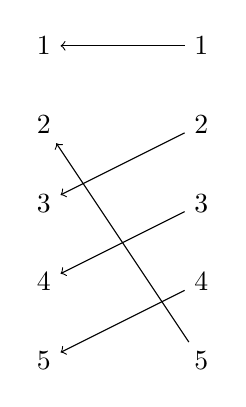
\begin{tikzpicture}
  \node (1a) at (2,4) {1}; \node (1b) at (0,4) {1};
  \node (2a) at (2,3) {2}; \node (2b) at (0,3) {2};
  \node (3a) at (2,2) {3}; \node (3b) at (0,2) {3};
  \node (4a) at (2,1) {4}; \node (4b) at (0,1) {4};
  \node (5a) at (2,0) {5}; \node (5b) at (0,0) {5};
  \draw [->] (1a) -- (1b);
  \draw [->] (2a) -- (3b);
  \draw [->] (3a) -- (4b);
  \draw [->] (4a) -- (5b);
  \draw [->] (5a) -- (2b);
\end{tikzpicture}
\caption{\label{fig:perm-a}A permutation on \(\{1,2,3,4,5\}\).}
\end{center}
\end{figure}

Viewing permutations this way gives the identity and inverse permutations a nice interpretation.
The identity map sends each element ``straight across'', and to find the inverse of \(\sigma\) simply reverse all the arrows.
We can also pronounce the \emph{composition} of functions as ``after''.
So, for instance, if \(\sigma\) and \(\tau\) are permutations of \(X\), then \(\tau \circ \sigma\) is pronounced ``tau after sigma'' -- meaning that to apply this map to a particular element of \(X\), we first apply sigma and then apply tau to the result.
Visually, this corresponds to plugging the output of \(\sigma\) to the input of \(\tau\) as in \autoref{fig:perm-b}.

\begin{figure}[h]
\begin{center}
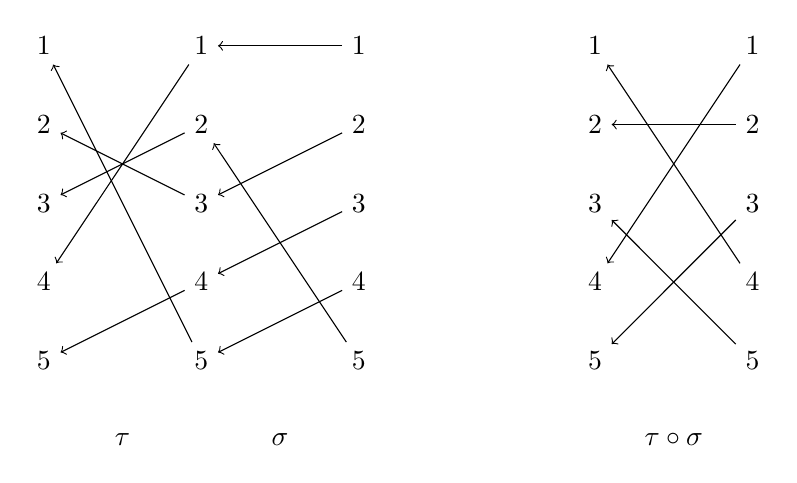
\begin{tikzpicture}
  \node (1a) at (2,4) {1}; \node (1b) at (0,4) {1}; \node (1c) at (-2,4) {1};
  \node (2a) at (2,3) {2}; \node (2b) at (0,3) {2}; \node (2c) at (-2,3) {2};
  \node (3a) at (2,2) {3}; \node (3b) at (0,2) {3}; \node (3c) at (-2,2) {3};
  \node (4a) at (2,1) {4}; \node (4b) at (0,1) {4}; \node (4c) at (-2,1) {4};
  \node (5a) at (2,0) {5}; \node (5b) at (0,0) {5}; \node (5c) at (-2,0) {5};
  \draw [->] (1a) -- (1b); \draw [->] (1b) -- (4c);
  \draw [->] (2a) -- (3b); \draw [->] (3b) -- (2c);
  \draw [->] (3a) -- (4b); \draw [->] (4b) -- (5c);
  \draw [->] (4a) -- (5b); \draw [->] (5b) -- (1c);
  \draw [->] (5a) -- (2b); \draw [->] (2b) -- (3c);
  \node at (1,-1) {$\sigma$}; \node at (-1,-1) {$\tau$};

  \node (1d) at (7,4) {1}; \node (1e) at (5,4) {1};
  \node (2d) at (7,3) {2}; \node (2e) at (5,3) {2};
  \node (3d) at (7,2) {3}; \node (3e) at (5,2) {3};
  \node (4d) at (7,1) {4}; \node (4e) at (5,1) {4};
  \node (5d) at (7,0) {5}; \node (5e) at (5,0) {5};
  \draw [->] (1d) -- (4e);
  \draw [->] (2d) -- (2e);
  \draw [->] (3d) -- (5e);
  \draw [->] (4d) -- (1e);
  \draw [->] (5d) -- (3e);
  \node at (6,-1) {$\tau \circ \sigma$};
\end{tikzpicture}
\caption{\label{fig:perm-b}Composition of permutations.}
\end{center}
\end{figure}

These arrow diagrams make it easy enough to visualize permutations, but they are a huge pain to compute with.
And so, we use an alternative notation instead, called \emph{cycle notation}.
Before we introduce cycle notation lets reconsider our arrow diagram in \autoref{fig:perm-a}.
There, we wrote down each element of \(X\) twice -- a bit redundant.
We can instead have only one copy of \(X\) as in \autoref{fig:perm-c}.

\begin{figure}[h]
\begin{center}
\begin{tikzpicture}
  \node (1) at (0:1)   {1};
  \node (2) at (72:1)  {2};
  \node (3) at (144:1) {3};
  \node (4) at (216:1) {4};
  \node (5) at (288:1) {5};
  \draw [->] (1) to [out=330,in=30,looseness=4] (1);
  \draw [->] (2) -- (3);
  \draw [->] (3) -- (4);
  \draw [->] (4) -- (5);
  \draw [->] (5) -- (2);
\end{tikzpicture}
\caption{\label{fig:perm-c}A permutation on \(\{1,2,3,4,5\}\).}
\end{center}
\end{figure}

Using this diagram it is less straightforward to see how to compose two permutations (though it can be done, say, by using different colors for the arrows of different permutations).
But it is easier to see what this permutation does when we apply it over and over.
2 goes to 3, 3 goes to 4, 4 goes to 5, and 5 goes to 2, while 1 goes to itself.
Cycle notation is just a compact way to express this diagram.
For instance, the permutation of \autoref{fig:perm-c} would be written in cycle notation as \[ (1)(2\ 3\ 4\ 5) \] or, more compactly, simply as \[ (2\ 3\ 4\ 5). \]
Lists of objects written inside parentheses are called \emph{cycles}\index{cycle notation}.
